%Dokumentklasse
\documentclass[a4paper,12pt, headings=small, bibtotoc, numbers=noenddot]{scrreprt} %bibtotoc = bibliography to table of contents, bindet Literaturverzeichnis in Inhaltsverzeichnis ein
\usepackage[left= 2.5cm,right = 2cm, top = 2cm, bottom = 2cm]{geometry} %Seitenränder
\usepackage[onehalfspacing]{setspace} %1,5 Zeilenabstand

% ============= Packages =============

% Dokumentinformationen
\usepackage[
	pdftitle={Titel der Arbeit},
	pdfsubject={Abschlussarbeit},
	pdfauthor={Max Mustermann},
	pdfkeywords={}
	pdftex=true, 
	colorlinks=true,
 	breaklinks=true,
	citecolor=black,
	linkcolor=black,	
	menucolor=black,	
	urlcolor=black,
]{hyperref}


% Standard Packages
\usepackage{libertine}	%Schriftart "Biolinum", Sans Serif
\renewcommand*\familydefault{\sfdefault} %Setzt die Standardschriftart auf Sans Serif
\usepackage[T1]{fontenc}
\usepackage{mathptmx} %Times new roman
\usepackage[utf8]{inputenc}
\usepackage[ngerman]{babel}
\AtBeginDocument{\renewcommand{\chaptername}{}}

\usepackage{rotating}
\usepackage{subfigure}
\usepackage{graphicx}
\graphicspath{{img/}}

\usepackage{multirow}
\usepackage{placeins}

\usepackage{fancyhdr}
\usepackage{lmodern}
\usepackage{color}
\usepackage{transparent}
\usepackage[justification=centering, singlelinecheck=false]{caption} %Damit die Tabellenbeschriftung zentriert steht
\usepackage{nomencl}
\usepackage{tabularx}
\usepackage{longtable}
\usepackage{booktabs}
\usepackage{pdfpages}
\usepackage{acronym}
\usepackage{setspace}

%Schriftgröße von section auf 12pt setzen
\addtokomafont{section}{\normalsize} 
\addtokomafont{chapter}{\large}
%Abbildungsbeschriftungen fett gedruckt einstellen
\addtokomafont{captionlabel}{\bfseries}


%Abstände zwischen Text und Überschriften
%Zeilenabstände bei Unterkapiteln
\RedeclareSectionCommand[beforeskip=18pt, afterskip=6pt]{section}
%Zeilenabstände bei Unter-unterkapiteln 
\RedeclareSectionCommand[beforeskip=12pt,afterskip=1pt]{subsection}
\RedeclareSectionCommand[%
  beforeskip=0pt,
  afterskip=1\baselineskip plus .1\baselineskip minus .167\baselineskip
]{chapter}


% zusätzliche Schriftzeichen der American Mathematical Society
\usepackage{amsfonts}
\usepackage{amsmath}

\usepackage{float} %erlaubt die Verwendung von H in Bildern
% mu im normalen Text: \textmu
\usepackage{textcomp}

\usepackage[backend=bibtex, style=alphabetic, uniquename=allfull, minalphanames=4, maxalphanames=4]{biblatex}
\addbibresource{Literatur.bib}

% nicht einrücken nach Absatz
\setlength{\parindent}{0pt}

\setcounter{secnumdepth}{4}
\setcounter{tocdepth}{4}

%url umbrechen
\usepackage{url}
\usepackage{microtype} %Sorgt für bessere Platzausnutzung der \hbox bei Umbruechen
\setlength{\emergencystretch}{1em} %Sorgt für bessere Platzausnutzung der \hbox bei Umbruechen

\setcounter{biburlnumpenalty}{100}
\setcounter{biburlucpenalty}{100}
\setcounter{biburllcpenalty}{100}
% ============= Package Einstellungen & Sonstiges ============= 

%römische Aufzählungen mit \RM{Zahl}
\newcommand{\RM}[1]{\MakeUppercase{\romannumeral #1}}

% ============= Dokumentbeginn =============

\begin{document}

\pagestyle{empty}   %leere Seite

%Seitennummerierung neu beginnen, Zahlen [arabic], röm.Zahlen [roman,Roman], Buchstaben [alph,Alph]

%Deckblatt
\label{Coversheet}
\begin{minipage}{0.5\textwidth}
\begin{flushleft}

\includegraphics[width=\textwidth]{chapter/Bilder/LKT_logo.png}
\end{flushleft}
\end{minipage}
\begin{minipage}{0.5\textwidth}
\begin{flushright}

\includegraphics[width=0.65\textwidth]{chapter/Bilder/UdS_Logo.png}
\end{flushright}
\end{minipage}
\headrule

\vspace{1.5cm}

\begin{center}
\LARGE \textbf{Vitamintablettenspender}\\ 
\vspace{3cm}
\textbf{Projektarbeit} \\
\Large Systementwicklungsmethodik 2\\ 
WS 2019/20\\
im Studiengang Systems Engineering\\
der Naturwissenschaftlich-Technischen Fakultät \\
der Universität des Saarlandes\\
\vspace{2.5cm}
\Large von\\
\vspace{1cm}
Kristian König und Tim Goll\\
Matrikelnummern: 2560270, 2553050 \\
Gruppennummer: 1\\
\vspace{1cm}
Saarbrücken, 2020
\end{center}
\newpage 

%Leerseite für doppelseitigen Druck
\thispagestyle{empty}
\quad 
\newpage

%Aufgabenstellung
%Hier wird die der verfassten Arbeit zugehörige Aufgabenstellung im PDF-Format eingebunden. Dazu wird im folgenden Block der Titel ,,Aufgabenstellung.pdf'' durch den entsprechenden Dateinamen ersetzt.
\label{Aufgabenstellung}

\includepdf[pages={1-5}]{chapter/Bilder/aufgabenstellung} 
\newpage

%Leerseite für doppelseitigen Druck
%\thispagestyle{empty}
%\quad 
%\newpage

%Eidestatliche Erklärung
%\label{Erklaerung}

%\begin{center} 
%\begin{minipage}[t]{120mm}
% \vspace{8cm}
%Ich versichere hiermit, dass ich die vorliegende Arbeit
%angegebenen Quellen und Hilfsmittel benutzt habe.\\  
%\end{minipage}
%\end{center}

%\vspace{3cm}
%Saarbrücken, den 30.04.2018  ~~~~~~~~~~~~~~~~~~~~~~~~~~~~~~~~~~~~~~~~~~~~~~~ Vorname Nachname
%\newpage

%Leerseite für doppelseitigen Druck
%\thispagestyle{empty}
%\quad 
%\newpage

\pagestyle{fancy} \newpage   %Seitenlayout normal
\fancyhf{} 
\fancyhead[L]{\nouppercase{{\fancyplain{}{\rightmark }}} } 
\fancyhead[R]{\thepage} 
\renewcommand{\headrulewidth}{0.5pt} 
\pagenumbering{Roman}


%Inhaltsverzeichnis
\clearpage \thispagestyle{empty}  ~ \clearpage \tableofcontents \thispagestyle{empty} \newpage

%Seitennummerierung neu beginnen, Zahlen [arabic], röm.Zahlen [roman,Roman], Buchstaben [alph,Alph]
\pagenumbering{arabic} \newpage
\renewcommand*{\chapterpagestyle}{empty}

%Einbinden aller .tex-Dateien, welche die einzelnen Kapitel beinhalten
\chapter{Lastenheft}

Es ist die Entwicklung eines innovativen Haushalt-Gadgets in AM-\&Multimaterial-Design vorgegeben. Dabei soll ein bedeutsames aber zeitgleich auch revolutionäres und innovatives Produkt entworfen werden. Vom Kunde ist ein Vitamintablettenspender gewünscht. Dieser soll über folgende Funktionen verfügen:
\begin{itemize}
\item Aufbewahrungsmöglichkeit für vier unterschiedliche Vitamintablettensorten
\item Automatischer Tablettenauswurf in einen Trinkbehälter
\item Automatisches Auffüllen des Trinkbehälters mit Wasser
\item Handlich
\item Leicht
\end{itemize}
Dazu wurden zusätzliche Kundenbefragungen und Umfragen hinsichtlich wünschenswerter Zusatzfunktionen durchgeführt. Als begeisternde Kriterien wurden folgende Wunschanforderungen formuliert:
\begin{itemize}
\item Touchdisplay zur Bedienung
\item Füllstandanzeige der Tablettenreservoirs
\item großer Wasserbehälter
\end{itemize}
Das Produkt soll dem Kunden im Februar 2020 mittels einem fertigen Prototypen vorgestellt werden.
% !TeX encoding = UTF-8
% !TeX root = ../Vitamintablettenspender.tex

\chapter{Konzeptionierung}

Im Entwicklungsprozess nimmt die Suche nach der optimalen Lösung für das vom Kunden gewünschte Produkt die Hauptaufgabe ein. Das Ergebnis soll nachvollziehbar und objektiv bewertbar sein. Dafür wird im Folgenden zunächst eine umfassende Planung des Produktes hinsichtlich Markt- und Wettbewerbschancen durchgeführt.

Die Entwicklung des Konzepts erfolgt darauffolgend anhand eines Projektplans, der den vom Kunden gewünschten Termin zur Vorstellung des Produktes mit einem Prototypen berücksichtigt. In der Anforderungsliste werden die Anforderungen des Kunden aus dem Lastenheft konkretisiert und durch interne Spezifikationen ergänzt. Damit wird eine Basis zur Entwicklung von Lösungsideen geschaffen.

Hierfür werden zunächst die Zusammenhänge von Anforderungen und Funktionen abstrakt in der Funktionsstruktur dargestellt, wobei das Loslösen vom Gegenständlichen und von vorzeitigen Festlegungen auf ein bestimmtes Lösungskonzept ermöglicht wird. Zur Systematisierung der Suche und Auswahl des optimalen Lösungsprinzips wird im morphologischen Kasten alle Lösungsoptionen aller Teilfunktionen berücksichtigt und verschiedene Gesamtlösungskombinationen unter Beachtung von Konflikten untereinander gebildet. Die abgesicherte Festlegung des zu realisierenden Lösungskonzeptes erfolgt in der Nutzwertanalyse. Zuletzt wird ein Grobentwurf zur Verdeutlichung des Wirkprinzips angefertigt.

\section{Produktplanung}

Marktanalysen, Wettbewerbsanalysen, Technologieanalysen und Patentanalyse


\section{Projektplan}

Für die Gestaltungsaufgabe mit Planung von

\begin{itemize}
\item Aufgaben
\item Dauer, Beginn und Ende der Aufgaben
\item Abhängigkeiten zwischen Aufgaben
\item ggf. kritischem Pfad
\end{itemize}

\section{Anforderungsliste}

\begin{itemize}
	\item Anforderungen des Lastenheftes präzisiert sowie um sinnvolle Anforderungen mund Angaben inkl. Verweis auf Lage im Kano-Diagramm ergänzt (min. 20 Anforderungen)
	\item Konsistenzmatrix für (min. 10) Hauptanforderungen
\end{itemize}

\newcolumntype{L}[1]{>{\raggedright\arraybackslash}p{#1}} % linksbündig mit Breitenangabe
\newcolumntype{C}[1]{>{\centering\arraybackslash}p{#1}} % zentriert mit Breitenangabe
\newcolumntype{R}[1]{>{\raggedleft\arraybackslash}p{#1}} % rechtsbündig mit Breitenangabe

\begin{longtable}{C{0.05\linewidth}C{0.05\linewidth}C{0.05\linewidth}L{0.75\linewidth}}
	\toprule
 	
 	\textbf{Nr.} & \textbf{F/W} & \textbf{Gew.} & \textbf{Beschreibung und Erläuterung}  \\
	
	\toprule
	\endfirsthead
	
	\textbf{1} & & & \textbf{Funktionsanforderungen}  \\
	1.1 & F & & Wirft gewünschte Vitamintablette aus  \\
	1.2 & W & & Tabletten werden automatisch ausgeworfen, wenn Glas platziert wird \\
	1.3 & W & & Immer nur eine der Tageszeit entsprechende Tablette darf ausgeworfen werden um Vitaminbalance zu garantieren \\
	1.4 & W & & Modernes Design \\
	1.5 & F & & Gute Standfestigkeit oder Möglichkeit zu Wandmontage \\
	1.6 & F & & Anzeige der aktuellen Uhrzeit \\
	1.7 & F & & Anzeige der nächsten Tablette mit deren Uhrzeit \\
	1.8 & F & & Einfache und intuitive Bedienung \\
	1.9 & W & & Nutzerprofile, sodass zwischen mehreren Nutzern gewechselt werden kann \\
	1.10 & F & & Vorrat-Leer Sensor um Nutzer auf Röhrchenwechsel hinzuweisen \\
	1.11 & W & & Warnton, wenn Tablette vergessen wurde \\
	
	\midrule
	
	\textbf{2} & & & \textbf{Mechanische/Geometrische Anforderungen} \\
	2.1 & F & & Muss kompatibel sein mit handelsüblichen Vitaminröhrchen \\
	2.2 & F & & Verwendung robuster Sensoren um Lebensdauer zu erhöhen \\
	2.3 & W & & Handliches Gewicht: $<\,5\,\text{kg}$ \\
	2.4 & W & & Maximale Abmessungen: $X\,\text{cm}\,\times\,Y\,\text{cm}\,\times\,Z\,\text{cm}$ \\
	
	\midrule
	
	\textbf{3} & & & \textbf{Sicherheitsanforderungen} \\
	3.1 & F & & Auswurfsmechanismus muss geschützt sein, sodass Finger nicht versehentlich hinein gerät \\
	3.2 & F & & Standfeste Position des Glases \\
	
	\midrule 
	
	\textbf{4} & & & \textbf{Umwelt- und Wartungsanforderungen} \\
	4.1 & F & & Verwendung von lebensmittelechten Materialien \\
	
	\midrule
	
	\textbf{5} & & & \textbf{Produktions- und Fertigungsanforderungen} \\
	5.1 & F & & Funktionsprototyp bis zum 07.02.2020 \\
	5.2 & W & & Verwendung wasserfester Materialien \\
	
	\midrule
	
	\textbf{6} & & & \textbf{Sonstiges} \\
	6.1 & F & & \\
	
	\bottomrule
	
	\caption{Anforderungsliste (F$\,=\,$Festanforderung, W$\,=\,$Wunschanforderung)}
	\label{anforderungsliste}
\end{longtable}


\section{Funktionsstruktur}

\begin{itemize}
	\item Allgemeine kybernetische Black-Box-Darstellung
	\item Hierarchische Funktionsstruktur (min. 10 Teilfunktionen)
	\item Funktionsmodell mit Darstellung der (min. 10) wichtigsten Funktionen
\end{itemize}


\section{Lösungsprinzipien}

\begin{itemize}
	\item Morphologischer Kasten mit (jeweils min. 4) Teillösungsprinzipien (ggf. durch geeignete Lösungsfindungsmethoden) für diese wichtigsten Funktionen
	\item Verträglichkeitsmatrix für die Teilprinzipien
	\item Kennzeichnung von min. 3 möglichen Gesamtlösungskombinationen im morphologischen Kasten
	\item Bewertung dieser Gesamtlösungskombinaitonen
\end{itemize}

\section{Technische Prinzipskizze}

Anfertigung einer technischen Prinzipskizze zur Verdeutlichung des Wirkprinzips
% !TeX encoding = UTF-8
% !TeX root = ../Vitamintablettenspender.tex

\chapter{Methodische Werkstoffauswahl}
Von der Produktentwicklung werden leistungsfähige Systeme bei gleichzeitiger Erfüllung von Sicherheits- und Umweltverträglichkeitsanforderungen erwartet. Steigenden Kosten für Material und Energie werden im Zuge des Multi-Material-Designs mittels einer methodischen Werkstoffauswahl durch die \glqq Ashby-Methode\glqq{} und den dabei entstehenden intelligenten Lösungen entgegengewirkt. Dabei werden unterschiedlichste Aspekte wie die Möglichkeit zur generativen Fertigung bzw. dem Additive Manufacturing berücksichtigt. Die Auslegung der Hauptkomponenten des Produktes unterliegt den jeweils gültigen Randbedingungen und ihren zu erfüllenden Funktionen und werden hinsichtlich ihrer freien Variablen untersucht und bezüglich der Werkstoffauswahl optimiert. Eine \glqq Performance-Rechnung\grqq{} ermöglicht die Einbeziehung von mathematischen und physikalischen Formeln zur Entmystifizierung der Werkstofffaktoren. In der kommerziellen Software CES Selector der Firma Granta Design Ltd. (Cambridge, Vereinigtes Königreich), die von Michael Ashby, dem Erfinder der Ashby-Methode, gegründet wurde, wird mittels einer computergestützten Datenbank auf Basis der Performance-Rechnung die fünf besten in Frage kommenden Werkstofflösungen mit ihren Materialindizees ermittelt, woraus die optimale Werkstofflösung durch \glqq weiche\grqq{} Faktoren resultiert.\\
Für die Anwendung der Ashby-Methode muss zunächst die Hauptfunktion des Bauteils bestimmt werden. Darauffolgend müssen Randbedingungen definiert werden, auf Basis derer ein Ziel zur Optimierung gesetzt wird. Dabei treten freie Variablen auf, die während des Designprozesses des Produktes variiert werden können. Die Randbedingungen liefern im Allgemeinen numerische Gleichungen die einen Performance-Index implizieren. Ein höherer Performance-Index bedeutet konventionell ein besseres Material.\\
Im Folgenden wird das Prinzip von Ashby zur Materialauswahl auf die vier Hauptkomponenten des Systems angewandt. Dabei handelt es sich zunächst um das Gehäuse, worin der Standfuß, die Rückwand sowie die Oberseite zusammengefasst werden. Ein weiteres Bauteil, das der Werkstoffoptimierung unterzogen wird, ist die Tablettenrutsche, an die die ausgeworfenen Tabletten übergeben und zum Trinkbehälter transportiert werden. Dritte Hauptkomponente stellt die rohrförmige, transparente Tablettenlagerung. Zum Schluss werden die Aktoren, welche sich aus Pleuelstangen und einem Tablettenschieber zusammensetzen untersucht.

\section{Standfuß und Gehäuse}\label{section:3.1}
Das Gehäuse inklusive des Standfußes sowie der Oberseite zum Anschrauben der übrigen Bauteile ist im Querschnitt zusammen mit den wesentlich angreifenden Lasten in Abb. \ref{fig:0301skizze} (a) dargestellt. Die Streckenlast $q_0$ fasst die Gewichtskräfte der Tablettenrutsche, der Aktoren sowie der Behälter für die Lagerung der Tabletten zusammen. Die Einspannung am unteren Ende symbolisiert die Lagerung des Bauteils an der Oberfläche. Eine geeignete Abstraktion des Systems wird durch die Reduzierung der Streckenlast sowie der Einspannung auf zwei resultierende Kräfte in \ref{fig:0301skizze} (a) beschrieben. Darin ist die Kraft $F_{res}$ die Resultierende aus der Streckenlast und greift im Schwerpunkt der Last an. Die Einspannung am unteren Ende reduziert sich zu der für die Berechnung wesentlichen vertikalen Komponente $F_{L,V}$. Unter Vernachlässigung des Eigengewichts des Bauteils gilt näherungsweise $F_{res}\,\approx\,F_{L,V}$. Die Werkstoffauswahl und die Optimierung einer Zielfunktion kann für den dargestellten kritischen Teil des Gehäuse stellvertretend für die gesamte Struktur vorgenommen werden.
\begin{figure}[H]
	\centering
	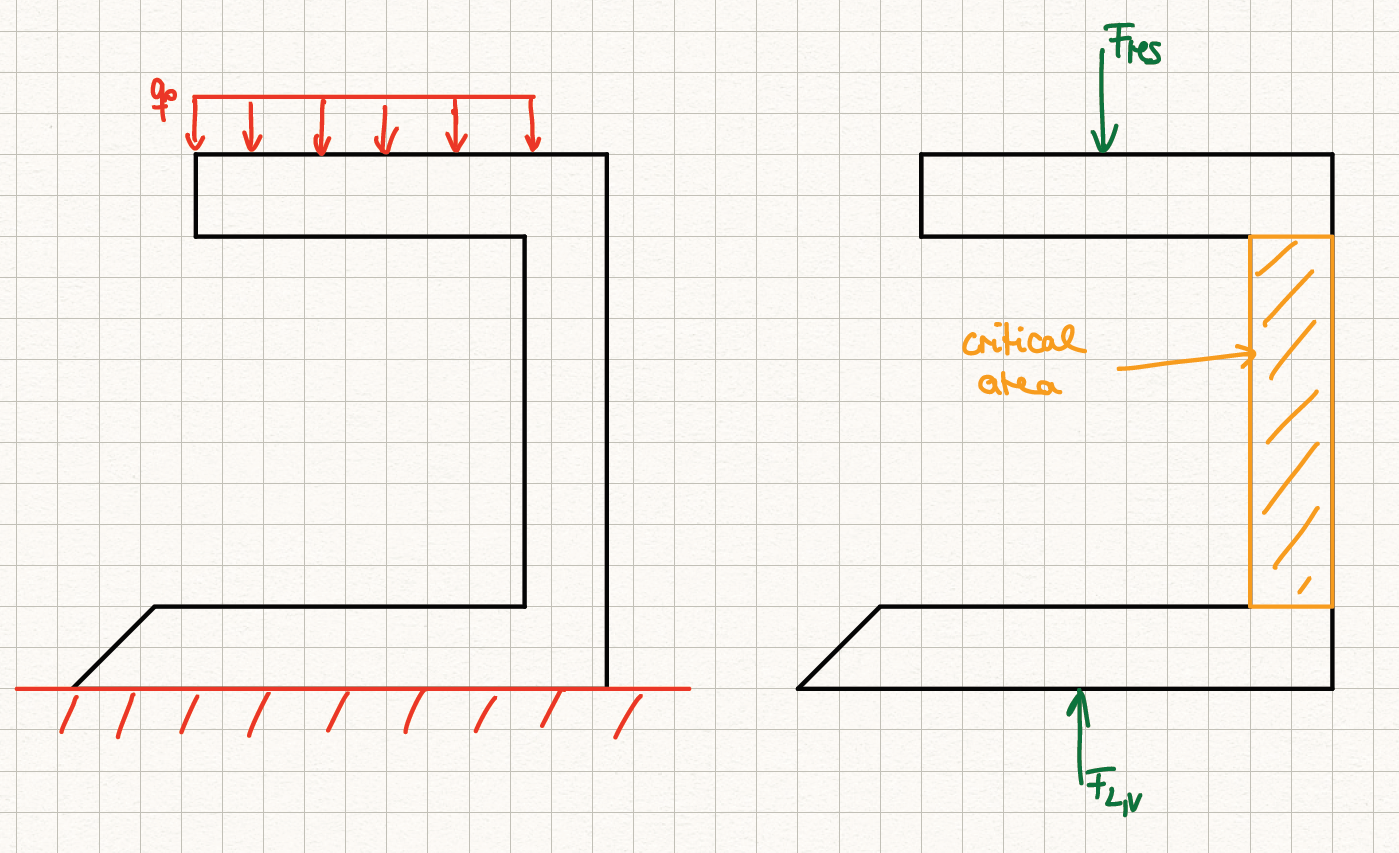
\includegraphics[width=1.0\linewidth]{chapter/Bilder/0301skizze}
	\caption{(a, links) Querschnittsdarstellung des Gehäuses und angreifende Lasten, (b, rechts) vereinfachte Darstellung mit angreifenden resultierenden Kräften und der kritischen Zone}
	\label{fig:0301skizze}
\end{figure}
\begin{figure}[H]
	\centering
	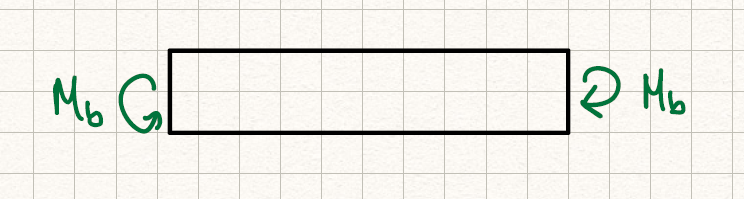
\includegraphics[width=1.0\linewidth]{chapter/Bilder/0301modell}
	\caption{Abstrahiertes Modell einer Platte unter reiner Biegung mit dem Biegemoment $M_b$}
	\label{fig:0301model}
\end{figure}
Dabei ist die \textbf{Funktion} des Bauteils die Tablettenrutsche, die Aktoren sowie die Tablettenbehälter zu stützen und in der Höhe zu halten. Auf Basis der Anforderungsliste in \ref{anforderungsliste} und der benötigten mechanischen Eigenschaften können folgende \textbf{Randbedingungen} definiert werden:
\begin{itemize}
	\item Material muss recyclebar sein
	\item Material muss ein guter Isolator sein, bzw. $\rho_e\,>\,10^{19}\,\mu\Omega$cm
	\item CO$_2$-Ausstoß bei der Materialgewinnung $\le\,2\,\frac{\text{kg}\,(\text{CO}_2)}{\text{kg}\,(\text{Material})}$
	\item Spezifische Festigkeit $\ge\,5\,\frac{\text{kN}\,\text{m}}{\text{kg}}$
	\item Bruchzähigkeit $\ge\,1\,\text{MPa}\,\sqrt{\text{m}}$
	\item Höhe des kritischen Teils/Länge der Platte $L\,=\,180\,$mm
	\item Biegesteifigkeit $S$ so, dass bei Einleitung der Kraft $F_{res}$ das an der Platte resultierende Biegemoment $M_b$ eine maximale Durchbiegung $w_{\text{max}}$ zur Folge hat
\end{itemize}
Das \textbf{Ziel} der Werkstoffauswahl ist die Reduzierung der Kosten für das Gehäuse. Als \textbf{freie Variablen} treten dabei zum einen die Querschnittfläche der rückwandigen Platte, welche durch Konzeptleichtbau im Verlauf des Produktdesigns optimiert werden kann, zum anderen die Wahl des Materials.
Dadurch, dass die Biegesteifigkeit $S$ sowie die Höhe der Platte $L$ vorgegeben sind, ergeben sich die beiden Gleichungen als Grundlage der Performance-Rechnung. Hierbei gilt zunächst für die Durchbiegung in der vertikalen Mitte der Platte ausgehend von der Differentialgleichung 2. Ordnung:
\begin{equation}
	E\,I\,w''(x)\,=\,-\,M_b\,
\end{equation}
durch zweifaches Integrieren, Umstellen und Einsetzen unter Vernachlässigung des Vorzeichens, das ausschließlich für die Richtung der Durchbiegung berücksichtigt werden muss, folgt:
\begin{equation} \label{durchbiegung}
	w\,\left(\frac{L}{2}\right)\,=\,\frac{M_b \,L^2}{8\,E\,I}\,\le\,w_{\text{max}},
\end{equation}
wobei $E\,I$ der Biegesteifigkeit $S$ entspricht. Als weitere Gleichung ergibt sich der Zusammenhang für die effektiven Kosten $K$, die in erster Linie über den Kostenfaktor $C_m$ mit der Masse der Platte korrelieren. Unter Berücksichtigung der Geometrie und der Materialdichte $\rho$ ergibt sich:
\begin{equation} \label{kosten}
	K\,=\,C_m\,m\,=\,C_m\,\rho\,A\,L\,.
\end{equation}
Dabei ist das Flächenträgheitsmoment eine Funktion der Querschnittfläche, die als rechteckig angenähert werden kann. Hier sind jedoch die Kantenlängen $h$ und $b$ variabel. Damit gilt für die Querschnittsfläche:
\begin{equation} \label{flächeninhalt}
A\,=\,h\,b
\end{equation}
sowie für das Flächenträgheitsmoment:
\begin{equation} \label{flächenträgheitsmoment}
I\,=\,\frac{h\,b^3}{12}\,.
\end{equation}
Einsetzen von \ref{flächenträgheitsmoment} in \ref{durchbiegung} und \ref{flächeninhalt} in \ref{kosten} liefert die Gleichungen:
\begin{equation} \label{eingesetzt}
	w_{\text{max}}\,\ge\,\frac{3\,M_b \,L^2}{2\,E\,h\,b^3}\,, \qquad
	K\,=\,C_m\,\rho\,h\,b\,L
\end{equation}
Eliminieren von $b$ führt in \ref{eingesetzt} schließlich zu
\begin{equation}\label{performance}
K\,=\,\underbrace{\left(\frac{3\,M_b\,L^5\,h^3}{2\,w_{\text{max}}}\right)^{\frac{1}{3}}}_{\text{konstanter Vorfaktor}}\,\frac{C_m\,\rho}{E^{\frac{1}{3}}}\,.
\end{equation}
Die \textbf{Zielfunktion} ist damit durch
\begin{equation} \label{performance31}
P_{\text{CR}}^{3.1}\,=\,\frac{1}{K}\,=\,\frac{E^\frac{1}{3}}{C_m\,\rho}
\end{equation}
definiert, wobei der Materialindex $P_{\text{CR}}^{3.1}$ zu maximieren ist. Dabei stellen hohe Werte von $P_{\text{CR}}^{3.1}$ einen idealen Kompromiss aus Kosten und Biegesteifigkeit dar.\\
Logarithmieren von \ref{performance31} liefert die Beziehung
\begin{equation}
\underbrace{3\,\ln(P_{\text{CR}}^{3.1})}_{=\,\text{konst.}}\,=\,\ln(E)\,-\,3\,\ln(C_m\,\rho)\,,
\end{equation}
wodurch sich mittels der Ashby-Methode in den Graph des logarithmierten Elastizitäsmodul über die logarithmierten Kosten eine Gerade der Steigung 3 legen lässt, welche einen variablen y-Achsenabstand in Abhängigkeit des Materialindex' aufweist, s. Abb. \ref{fig:ces_3_1_1}.\\
\begin{figure}[H]
	\centering
	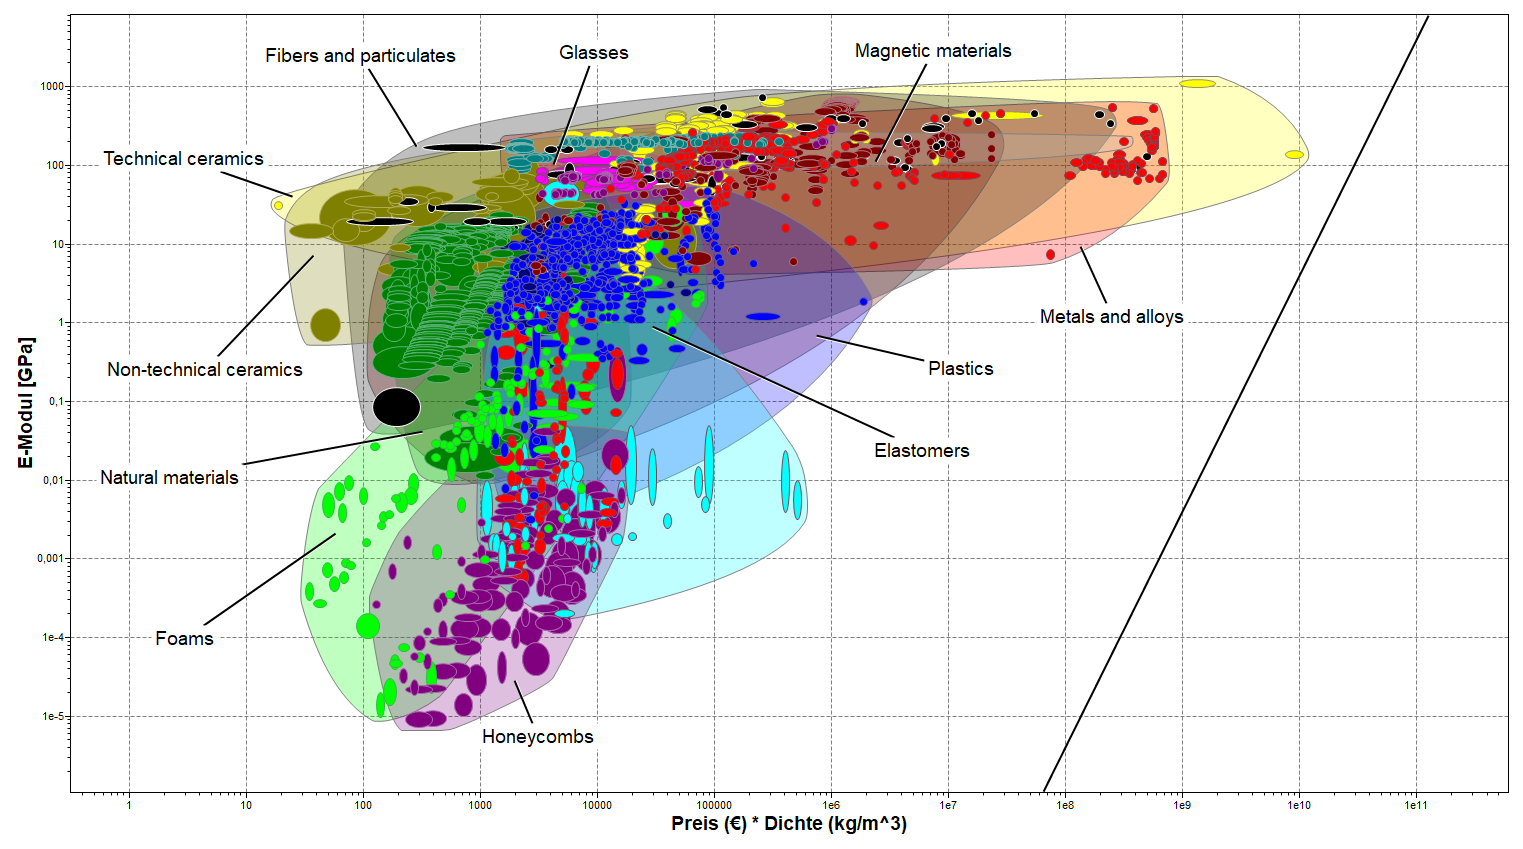
\includegraphics[width=1.0\linewidth]{chapter/Bilder/3_1_1}
	\caption{Caption TODO}
		\label{fig:ces_3_1_1}
\end{figure}
Hinzufügen der Randbedingungen \glqq recyclebar\grqq{} und \glqq guter Isolator\grqq{} eliminiert einige Materialien und führt zur graphischen Darstellung in Abb. \ref{fig:ces_3_1_2}.\\
\begin{figure}[H]
	\centering
	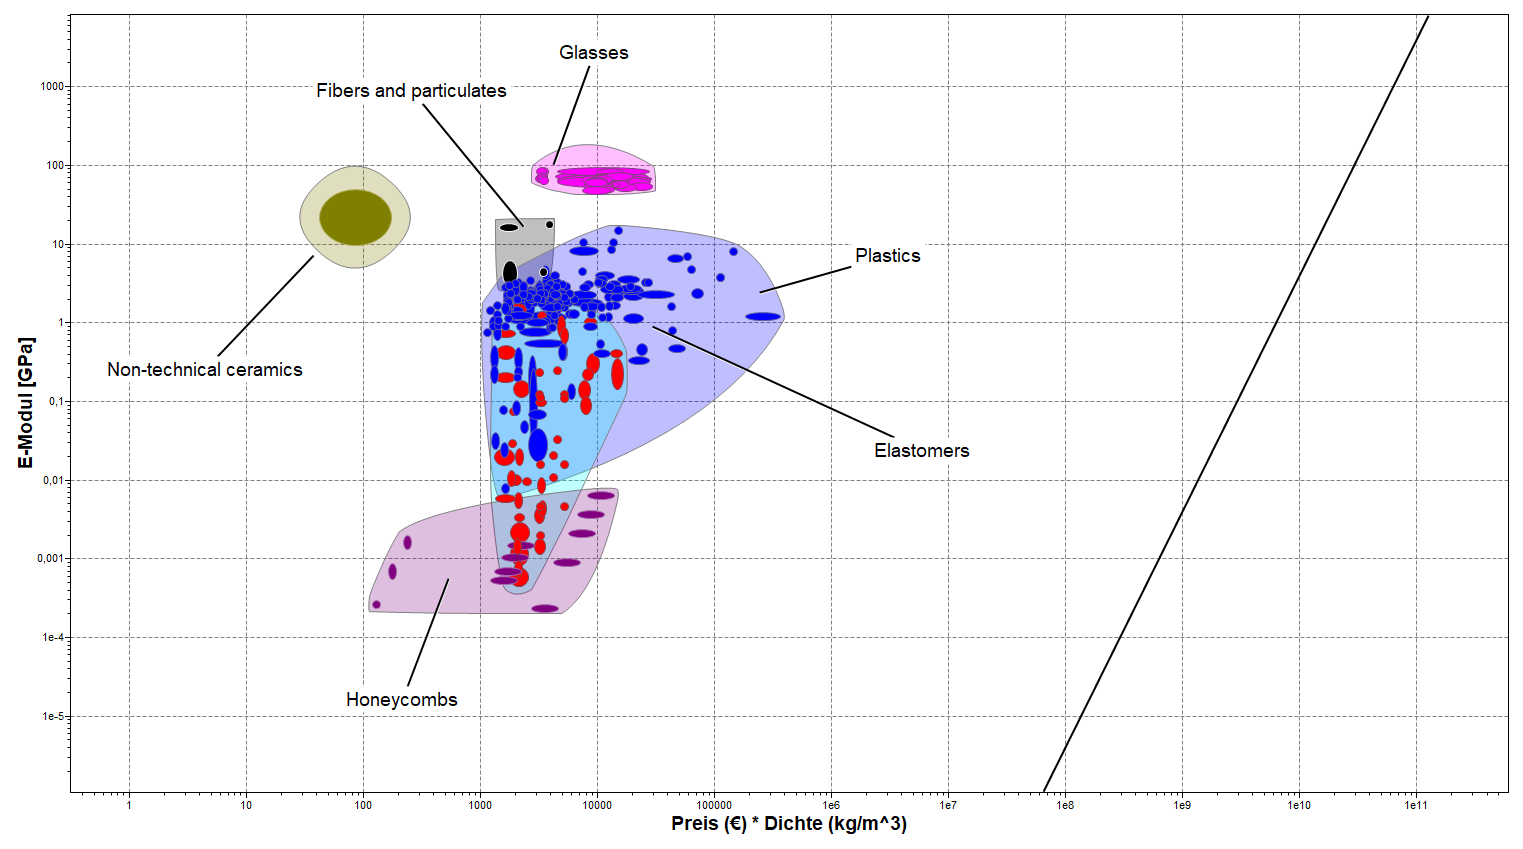
\includegraphics[width=1.0\linewidth]{chapter/Bilder/3_1_2}
	\caption{Caption TODO}
	\label{fig:ces_3_1_2}
\end{figure}
Unter Berücksichtigung der übrigen Randbedingungen hinsichtlich des CO$_2$-Ausstoßes und der mechanischen Materialeigenschaften scheiden weitere Materialien aus (Abb. \ref{fig:ces_3_1_3}).\\
\begin{figure}[H]
	\centering
	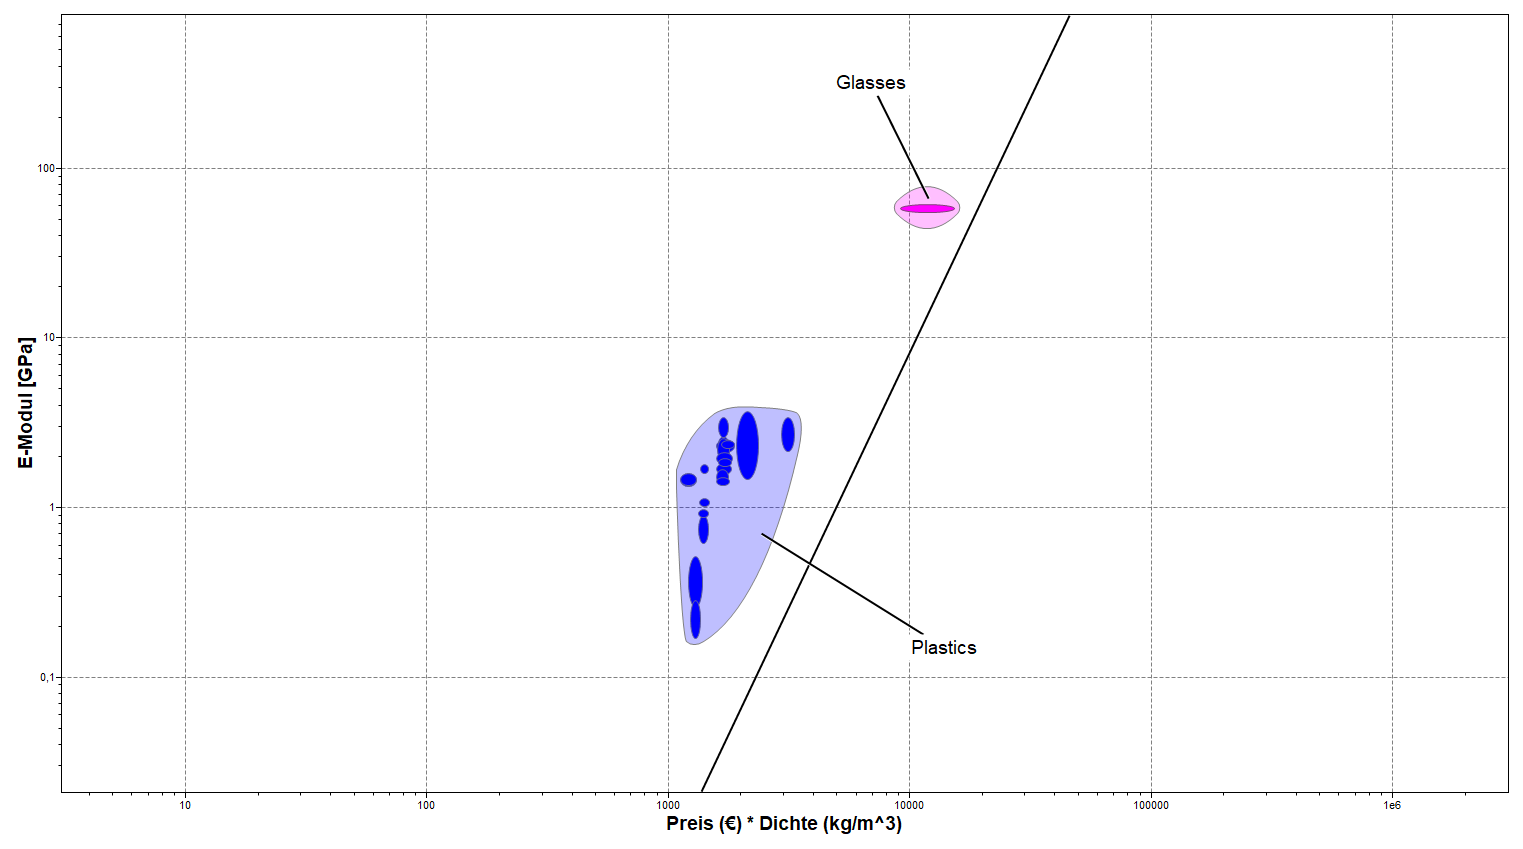
\includegraphics[width=1.0\linewidth]{chapter/Bilder/3_1_3}
	\caption{Caption TODO}
	\label{fig:ces_3_1_3}
\end{figure}
Erhöhung des y-Achsenabschnittes der Gerade führt zur Vernachlässigung aller Materialien, die unterhalb der Geraden liegen. Das am besten geeignete Material wird zuletzt von der Gerade eliminiert und weist den höchsten Performance-Index $P_{\text{CR}}^{3.1}$ auf (Abb. \ref{fig:ces_3_1_4})\\
\begin{figure}[H]
	\centering
	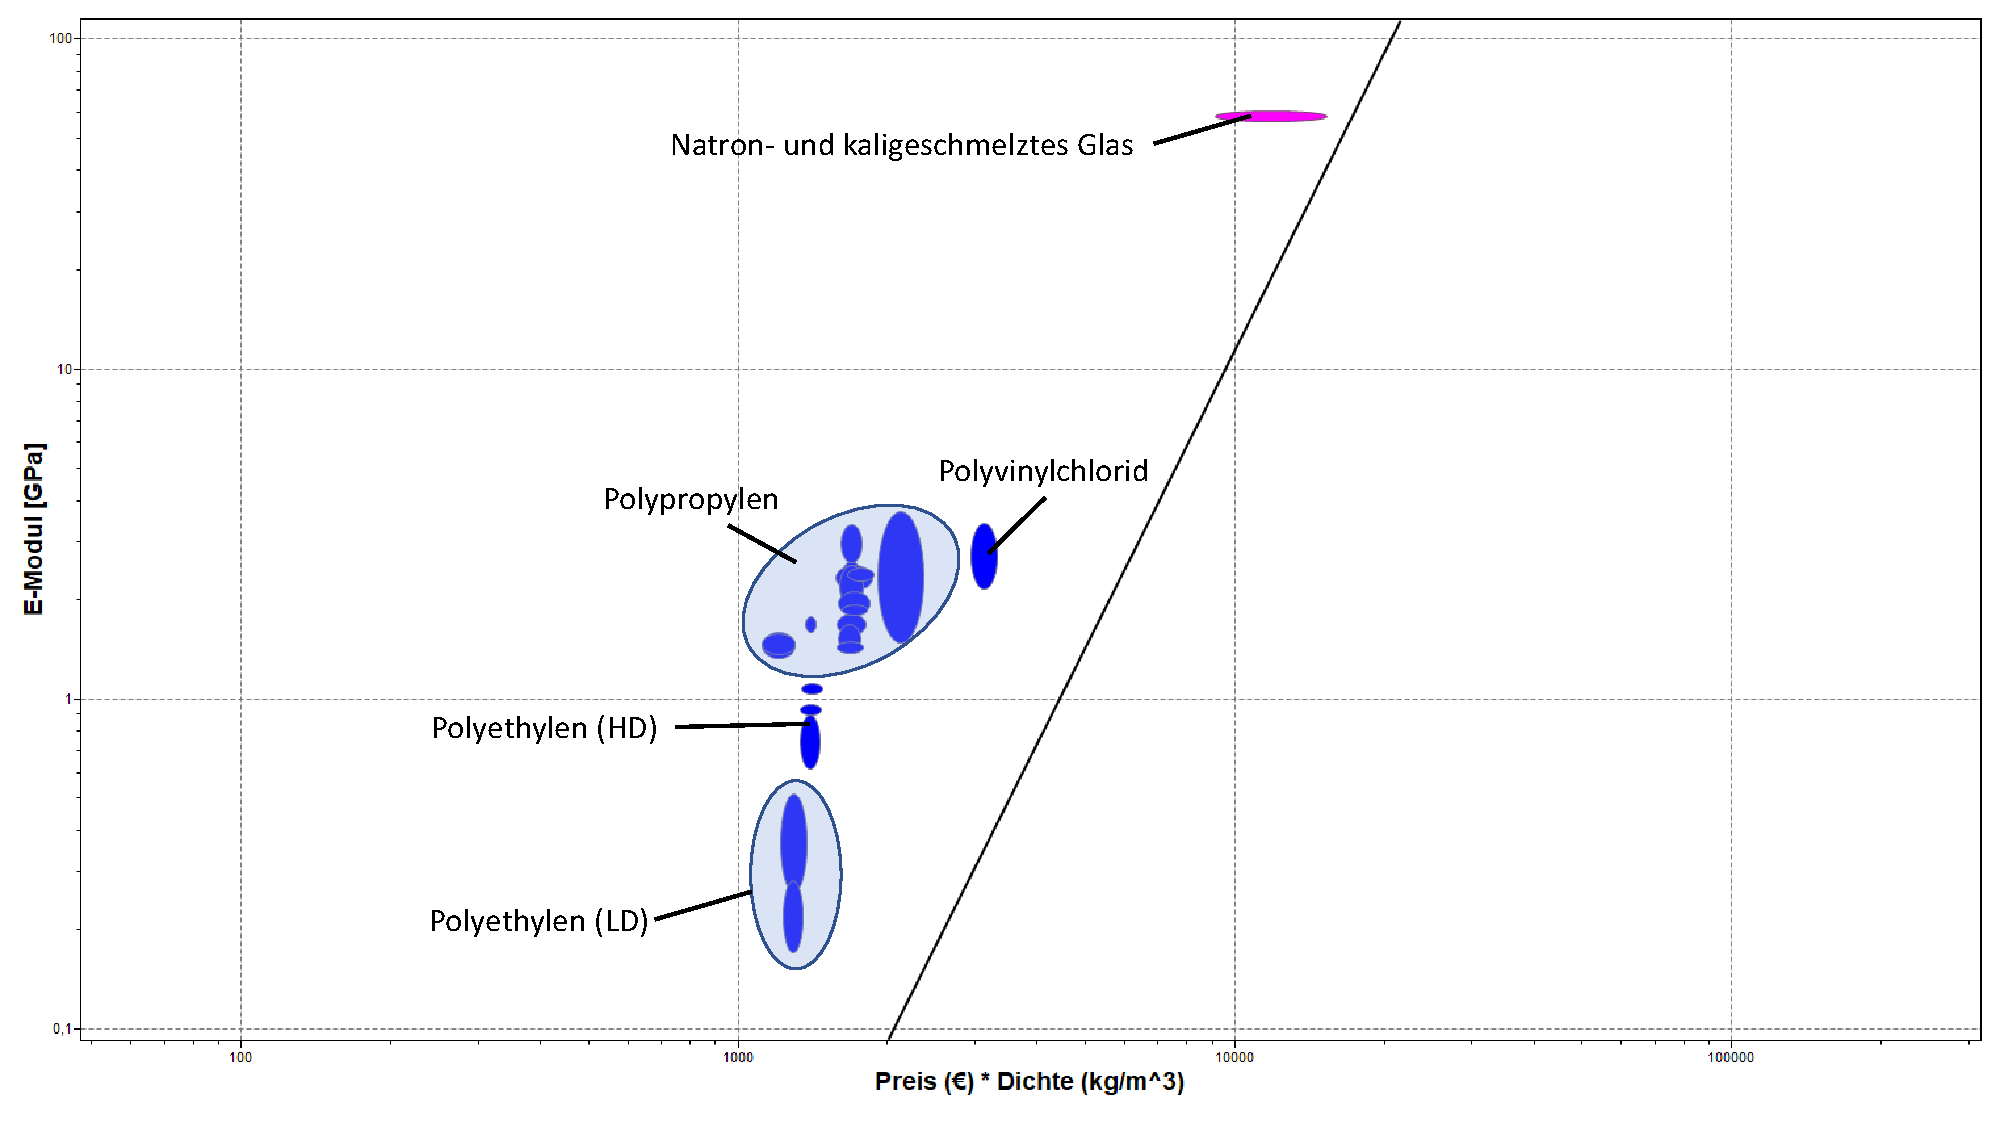
\includegraphics[width=1.0\linewidth]{chapter/Bilder/3_1_4}
	\caption{Caption TODO}
	\label{fig:ces_3_1_4}
\end{figure}
Die fünf geeignetsten Materialien werden dadurch ausfindig gemacht, dass sie zuletzt von der Gerade eliminiert werden und damit den höchsten Performance-Index besitzen. Für das betrachtete Problem ergibt sich:
\begin{itemize}
\item[1)] Polypropylen (PP, Materialindex: 9,46$\,\times10^{-4}$)
\item[2)] Polyethylen (PE, HD - high density, 7,3$\,\times10^{-4}$)
\item[3)] Polyethylen (PE, LD - low density, 5,55$\,\times10^{-4}$)
\item[4)] Polyvinylchlorid (PVC, 4,48$\,\times10^{-4}$)
\item[5)] Natron- und kaligeschmelztes Glas (3,3$\,\times10^{-4}$)
\end{itemize}
Dementsprechend fällt ohne weitere Einschränkung oder offensichtliche Nachteile die Wahl des Materials für das Gehäuse auf Polypropylen.

\section{Tablettenrutsche}
Die Tablettenrutsche besitzt die wesentliche \textbf{Funktion} die aus der Lagerung geschobenen Vitamintabletten mittels Schwerkraft entlang einer Bahn in ein bereitgestellten Trinkbehälter zu überführen. Sie wird direkt an das Gehäuse geschraubt und an ihr sind mehrere elektronische Bauteile wie u.a. Taster und die Servomotoren befestigt, daher erfährt hier die elektrische Resistivität eine erhöhte Bedeutung. Für die Werkstoffauswahl liegen insgesamt folgenden \textbf{Randbedingungen} vor:
\begin{itemize}
	\item Material muss recyclebar sein
	\item Material muss generativ bzw. additiv fertigbar sein
	\item Material muss ein guter Isolator sein, bzw. $\rho_e\,>\,10^{19}\,\mu\Omega$cm
	\item Plattengeometrie: Trapezförmiger Querschnitt (gleichschenklig und symmetrisch, Höhe $h\,=\,40\,$mm, Dicke $3\,=\,mm$
\end{itemize}
Das \textbf{Ziel} der Werkstoffwahl liegt in der Minimierung des CO$_2$-Ausstoßes bei der Materialgewinnung unter Erfüllung der minimalen spezifischen Bruchfestigkeit, die gewährleistet, dass trotz der hohen Zahl an Auswurfzyklen der Tabletten und dem dabei wirkenden Biegemoment die Bauteilstruktur nicht beeinflusst wird und keine Risse an der Oberfläche auftreten. \textbf{Freie Variable} ist in dem Auslegungsprozess die Wahl des Materials sowie die Längen $l_1$ und $l_2$ der beiden Grundseiten der Trapezquerschnittsfläche.\\
Aufgrund der vorgegebenen Plattengeometrie (s. Abb ?? a) gilt für den CO$_2$-Ausstoß beim Materialgewinnung in Abhängigkeit der Masse
\begin{equation}\label{masse32}
\text{CO}_2^{ges}\,=\,\text{CO}_2^F\,m\,=\,\text{CO}_2^F\,\rho\,V\,=\,\text{CO}_2^F\,\rho\,\frac{1}{2}\,(l_1\,+\,l_2)\,h\,d\,.
\end{equation}
Für die Normalspannung in der Randfaser der Platte gilt
\begin{equation}
\sigma\,=\,\frac{M_b}{I}\,z\,.
\end{equation}
Dabei ist $M_b$ das Biegemoment, $I$ das Flächenträgheitsmoment und $z$ der Abstand der Randfaser von der neutralen Faser. Damit an der Oberfläche des Bauteils keine Risse auftreten, darf wie in Abb. ?? die Spannung $\sigma$ nicht die Bruchfestigkeit $\sigma_f$ überschreiten
\begin{equation}\label{bruchfestigkeit32}
\sigma\,=\,\frac{M_b}{I}\,z\,\le\,\sigma_f\,.
\end{equation}
Es folgt für das Biegemoment aufgrund des in Abb. ?? b) dargestellten Lastfalls
\begin{equation}\label{lastfall32}
M\,=\,F\,\cos(45)\,h=\,F\,\frac{\sqrt{2}}{2}\,h\,.
\end{equation}
Unter Berücksichtigung der Plattengeometrie gilt für den Abstand $z$ der Randfaser zur neutralen Faser
\begin{equation}\label{geometrie32}
z\,=\,\frac{d}{2}\,.
\end{equation}
Das Flächenträgheitsmoment des Querschnittes entspricht im Krafteinleitungspunkt:
\begin{equation}\label{flächen32}
I\,=\,\frac{\frac{1}{2}\,(l_1\,+\,l_2)\,d^3}{12}\,=\frac{(l_1\,+\,l_2)\,d^3}{24}\,.
\end{equation}
Einsetzen von \ref{lastfall32}, \ref{geometrie32} und \ref{flächen32} in \ref{bruchfestigkeit32} liefert
\begin{equation}\label{eingesetzt32}
\sigma_f\,\ge\,\frac{24\,\sqrt{2}\,F}{4\,(l_1\,+l_2)\,d^3}\,h\,d\,=\,\frac{6\,\sqrt{2}\,F\,h}{(l_1\,+\,l_2)d^2}\,.
\end{equation}
Schlussendlich führt Eliminierung der freien Variable $(l_1\,+\,l_2)$ in \ref{masse32} und \ref{eingesetzt32} auf
\begin{equation}
\frac{2\,\text{CO}_2^{ges}}{\text{CO}_2^F\,\rho\,h\,d}\,=\,\frac{6\sqrt{2}\,F\,h}{d^2\,\sigma_f}\,.
\end{equation}
Der gesamte CO$_2$-Ausstoß lässt sich dadurch mit
\begin{equation}
\text{CO}_2^{ges}\,=\,\underbrace{\frac{3\,\sqrt{2}\,F\,h^2}{d}}_{\text{konstanter Vorfaktor}}\,\frac{\text{CO}_2^F\,\rho}{\sigma_f}
\end{equation}
berechnen.
Damit ergibt sich die Performance-Gleichung
\begin{equation} \label{zielfkt32}
P_{\text{CR}}^{3.2}\,=\,\frac{1}{\text{CO}_2^{ges}}\,=\,\frac{\sigma_f}{\text{CO}_2^F\,\rho}\,,
\end{equation}
deren Materialindex $P_{\text{CR}}^{3.2}$ zu maximieren ist.\\
Analog zu der in \ref{section:3.1} beschrieben graphischen Umsetzung mittels der Ashby-Methode lässt sich die logarithmierte spezifische Bruchfestigkeit über dem Logarithmus des Produktes von CO$_2$-Fußabdruck und Materialdichte auftragen.\\
\begin{figure}[H]
	\centering
	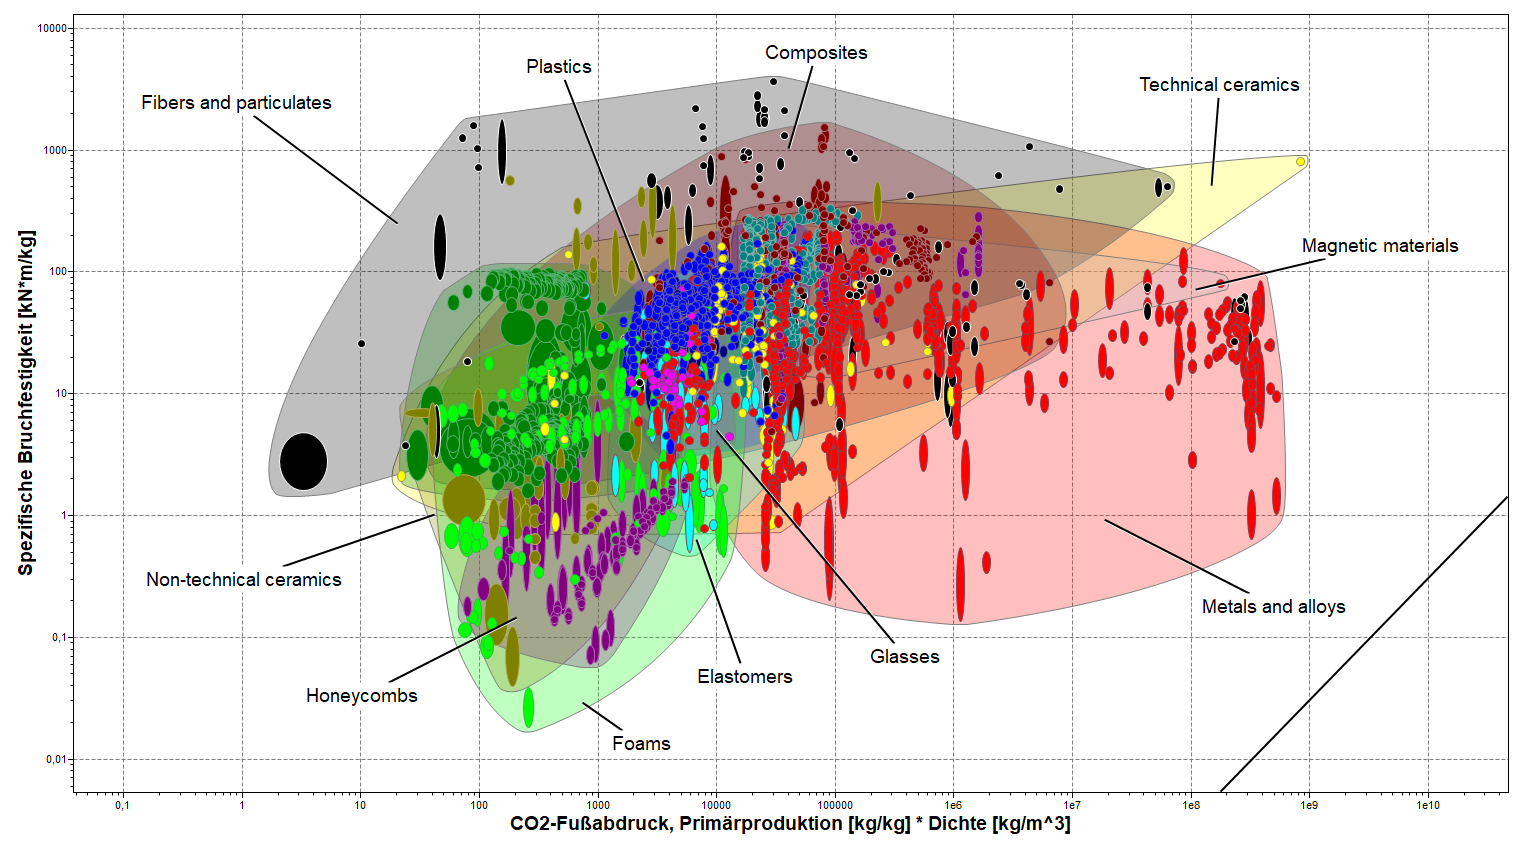
\includegraphics[width=1.0\linewidth]{chapter/Bilder/3_2_1}
	\caption{Caption TODO}
	\label{fig:ces_3_2_1}
\end{figure}
Hinzufügen aller Randbedingungen eliminiert einige Materialien, s. Abb. \ref{fig:ces_3_2_2}\\
\begin{figure}[H]
	\centering
	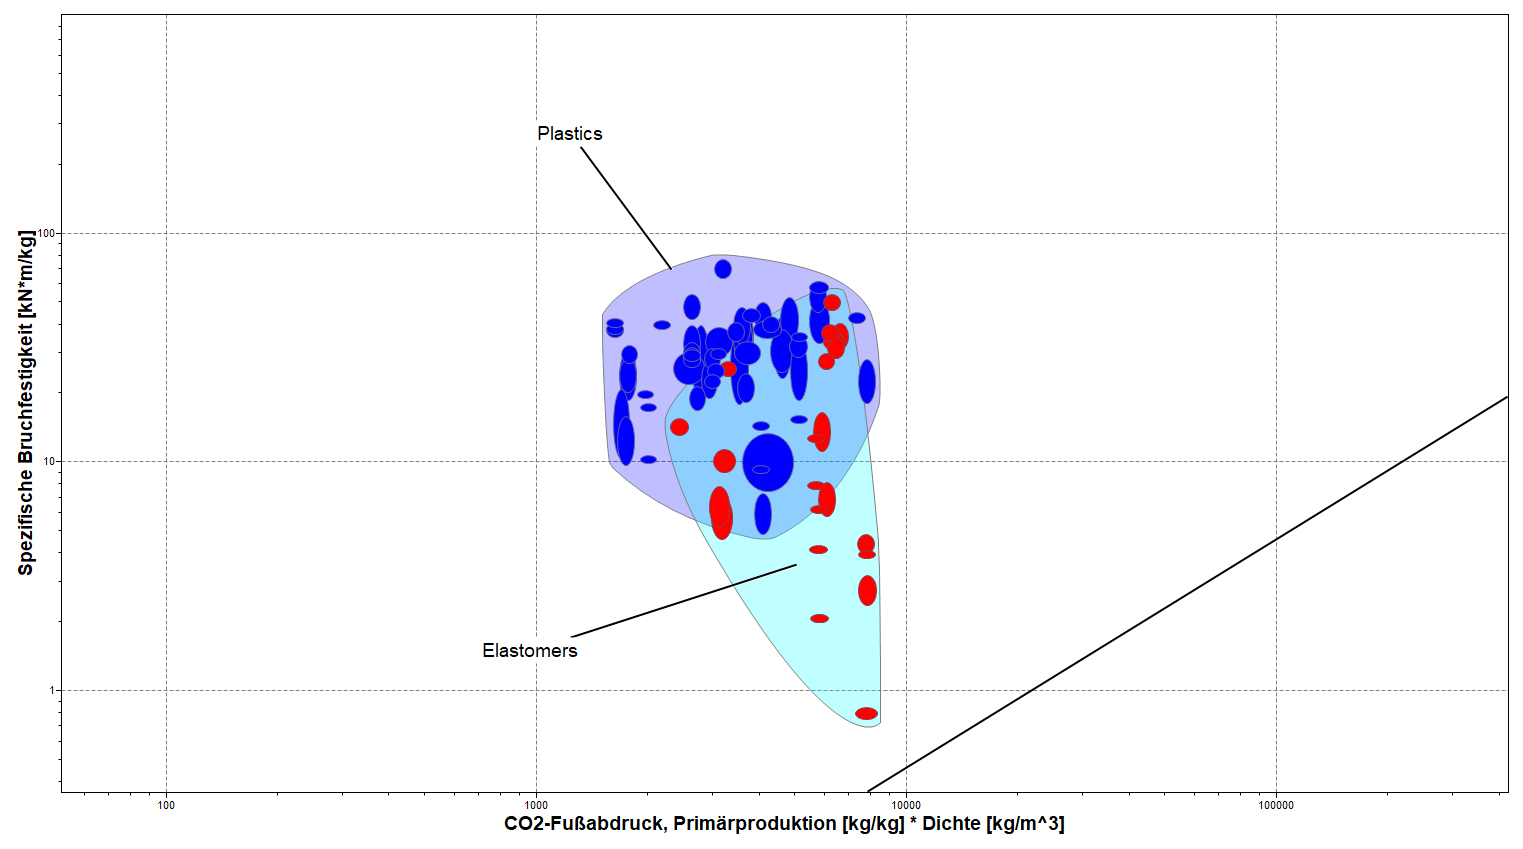
\includegraphics[width=1.0\linewidth]{chapter/Bilder/3_2_2}
	\caption{Caption TODO}
	\label{fig:ces_3_2_2}
\end{figure}
Verschieben der Gerade in positive y-Richtung liefert die am besten geeigneten Materialien. (Abb. \ref{fig:ces_3_2_3})\\
\begin{figure}[H]
	\centering
	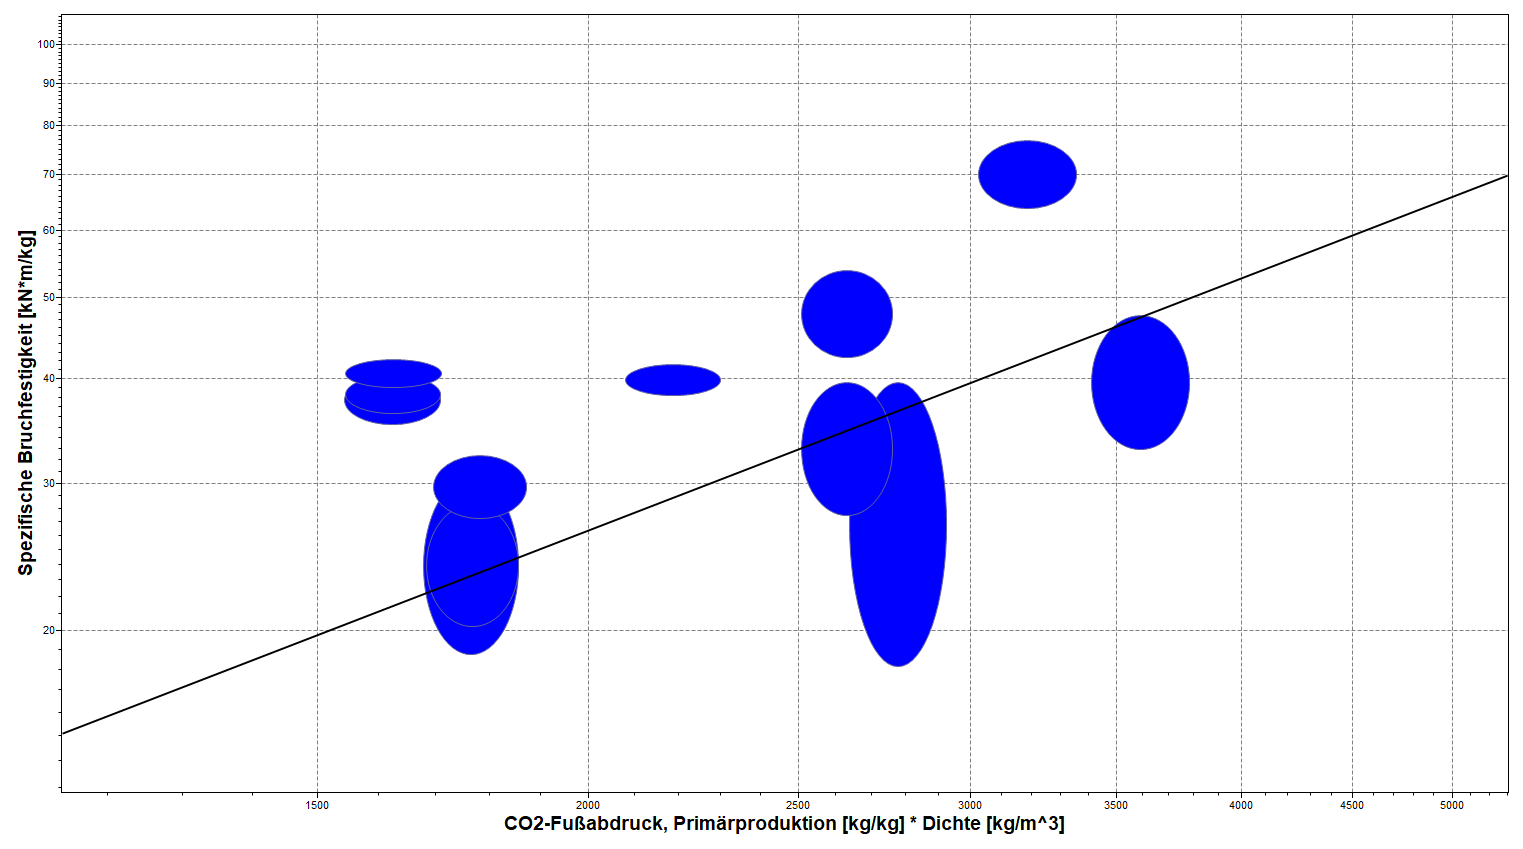
\includegraphics[width=1.0\linewidth]{chapter/Bilder/3_2_3}
	\caption{Caption TODO}
	\label{fig:ces_3_2_3}
\end{figure}
Die fünf dadurch ausgemachten geeignetsten Materialien lauten:
\begin{itemize}
	\item[1)] Polypropylen (PP, Materialindex: 0,025)
	\item[2)] Styrol-Acrylnitril (SAN, 0,022) 
	\item[3)] Polystyrol (PS, 0,0182)
	\item[4)] Polyethylen (PE, HD - high density, 0,0167)
	\item[5)] Acrylnitril-Butadien-Styrol (ABS, 0,011)
\end{itemize}
Da in \ref{section:3.1} bereits Polypropylen als das bestmögliche Material für das Gehäuse gewählt wurde, fällt die Wahl für die Tablettenrutsche ebenfalls auf PP. Das Material ist sehr gut geeignet für Anwendungen im Lebensmittelbereich, was die Entscheidung stützt.

\section{Tablettenlagerung}
Die Tablettenlagerung besteht aus Hohlzylindern, die direkt an die Tablettenrutsche geschraubt werden. Die \textbf{Funktion} dieses Bauteils stellt das sichere Lagern der Vitamintabletten sowie dem Zulassen einer optischen Prüfung des Füllstandes dar. Zur Erfüllung dieser Funktion sind folgende \textbf{Randbedingungen} gegeben:
\begin{itemize}
	\item Material muss recyclebar sein
	\item Material muss durchsichtig/transparent sein
	\item CO$_2$-Ausstoß bei der Materialgewinnung $\le\,2\,\frac{\text{kg}\,(\text{CO}_2)}{\text{kg}\,(\text{Material})}$
	\item Preis $\le\,2\,\frac{\text{€}}{\text{kg}}$
	\item Steifigkeit: Kein Umknicken bei Befüllung
	\item Festigkeit: Keine plastische Verformung bei Befüllung
	\item Bauteilhöhe $l\,=\,200\,$mm
	\item Innenradius des Lagerungsrohrs $r\,=\,14\,$mm
\end{itemize}
Das \textbf{Ziel} der Werkstoffauswahl ist die Minimierung der grauen Energie bei der Materialgewinnung für eine ausreichende Biegesteifigkeit. \textbf{Freie Variable} ist die Wahl des Materials sowie der Außenradius $R$ des Rohrs. Der Belastungszustand unter dem das Bauteil steht, ist in Abbildung ?? dargestellt. Dabei wird das Rohr an der Unterseite fest eingespannt und während des Befüllvorgangs unter Knickung an der Oberkante belastet.\\
Abbildung Belatungszustand\\
Die während der Primärproduktion verbrauchte Energie ist mit
\begin{equation}\label{energie33}
H^{ges}\,=\,H_p\,m\,=\,H_p\,\rho\,l\,A\,=\,H_p\,\rho\,l\,\pi\,\left(R^2\,-\,r^2\right)\,\approx\,c_1\,H_p\,\rho\,l\,\pi\,R^2
\end{equation}
definiert. Da der Innenradius $r$ bekannt ist, kann er näherungsweise durch einen konstanter Vorfaktor in der Rechnung ausgetauscht werden.\\
Da es sich bei dem gegebenen Lastfall, um die Knickung eines Rohres handelt, kann näherungsweise die Theorie des Eulerschen Knickstabes herangezogen werden. Dadurch lässt sich die kritische Last $F_{krit}$, bei der es zum Knick kommt, mit
\begin{equation}\label{fkrit33}
F_{krit}\,=\,\frac{\pi^2\,E\,I}{l^2}\,\ge\,F\,,
\end{equation}
berechnen, wobei die real-angreifende Last $F$ geringer sein muss.
Das Flächenträgheitsmoment für den Rohrquerschnitt ist durch
\begin{equation}\label{flächen33}
I\,=\,\frac{\pi}{4}\,\left(R^4\,-\,r^4\right)\,\approx\,c_2\,\frac{\pi}{4}\,R^4
\end{equation}
definiert. Auch hier geht $r$ nur als Konstante mit ein und kann in einem Produktausdruck durch einen weiteren konstanten Faktor $c_2$ ersetzt werden. Einsetzen von \ref{flächen33} in \ref{fkrit33} liefert
\begin{equation}
F\,\le\,\frac{\pi^2\,E\,c_2\,\frac{\pi}{4}\,R^4}{l^2}\,=\,\frac{c_2\,\pi^3\,E\,R^4}{4\,l^2}\,.
\end{equation}
Eliminieren der freien Variable $R$ führt schließlich im Grenzfall $F\,=\,F_{krit}$ zu
\begin{equation}
F\,=\,\frac{c_2\,\pi^3\,E\,R^4}{4\,l^2}\,=\,\frac{c_2\,\pi^3\,E\,H_{ges}^2}{4\,c_1^2\,l^2\,H_p^2\,\rho^2\,l^2\,\pi}\,=\,\frac{c_2\,\pi\,E\,H_{ges}^2}{4\,c_1^2\,l^3\,\rho^2\,H_p^2}\,.
\end{equation}
Die gesamt aufgewendete Energie in der Produktion lässt sich damit durch
\begin{equation}
H_{ges}\,=\,\underbrace{\left(\frac{4\,c_1^2\,l^3\,F}{c_2\,\pi}\right)^\frac{1}{2}}_{\text{konstanter Vorfaktor}}\,\frac{\rho\,H_p}{E^\frac{1}{2}}
\end{equation}
berechnen.
Es ergibt sich die Performance-Gleichung
\begin{equation} \label{zielfkt3}
P_{\text{CR}}^{3.3}\,=\,\frac{1}{H_{ges}}\,=\,\frac{E^\frac{1}{2}}{H_p\,\rho}\,,
\end{equation}
deren Materialindex $P_{\text{CR}}^{3.3}$ zu maximieren ist. Die graphische Darstellung der logarithmierten Gleichung \ref{zielfkt3} ist in Abb. ?? ersichtlich. Darin sind die verschiedenen Materialien eingetragen.\\
\begin{figure}[H]
	\centering
	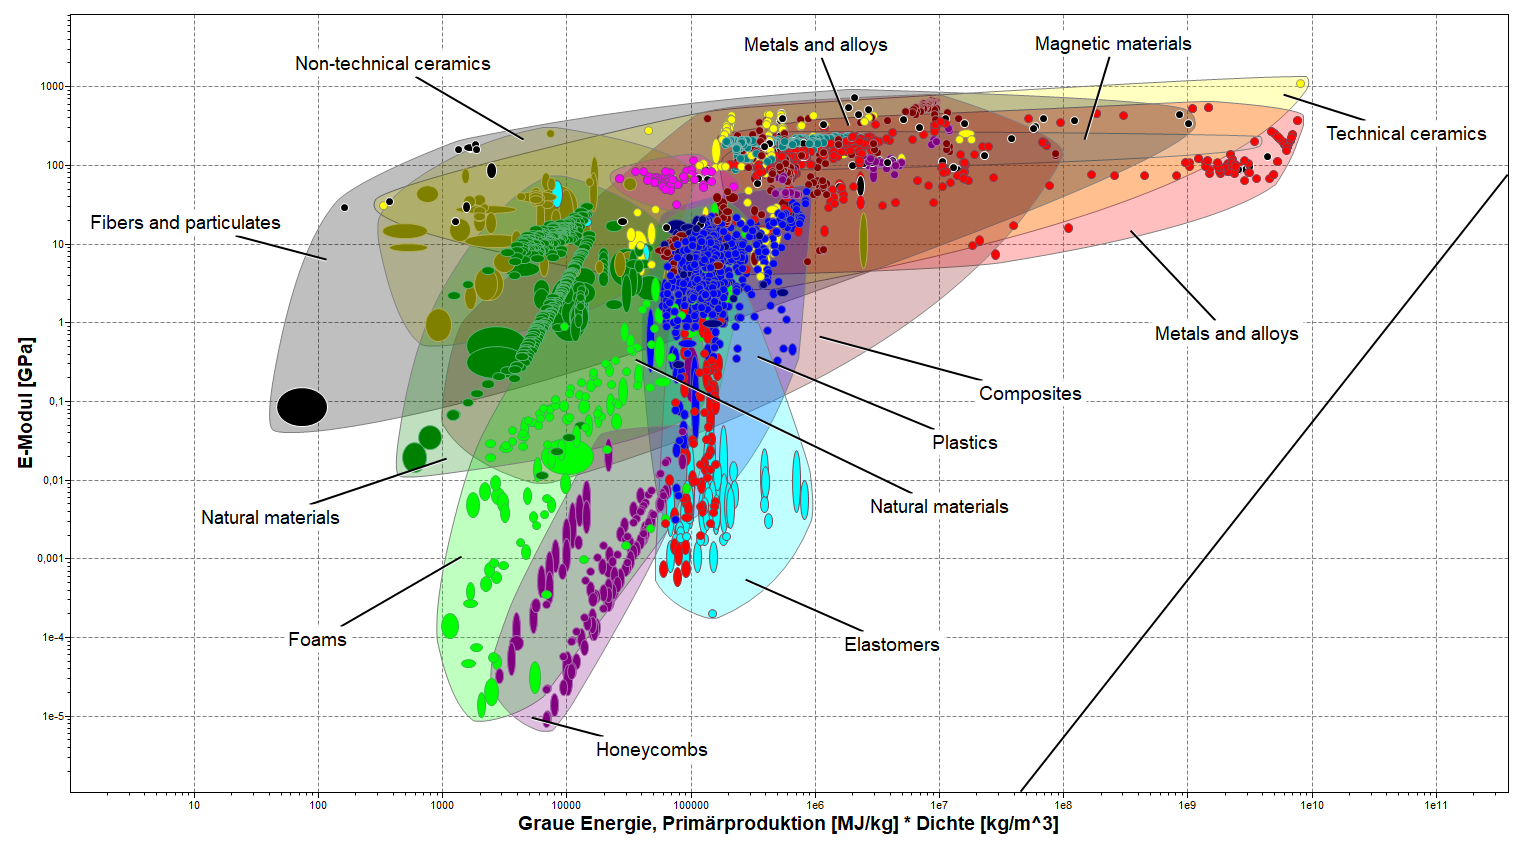
\includegraphics[width=1.0\linewidth]{chapter/Bilder/3_3_1}
	\caption{Caption TODO}
	\label{fig:ces_3_3_1}
\end{figure}
Hinzufügen aller Randbedingungen schließt einige Materialien aus, Abb. \ref{fig:ces_3_3_2}\\
\begin{figure}[H]
	\centering
	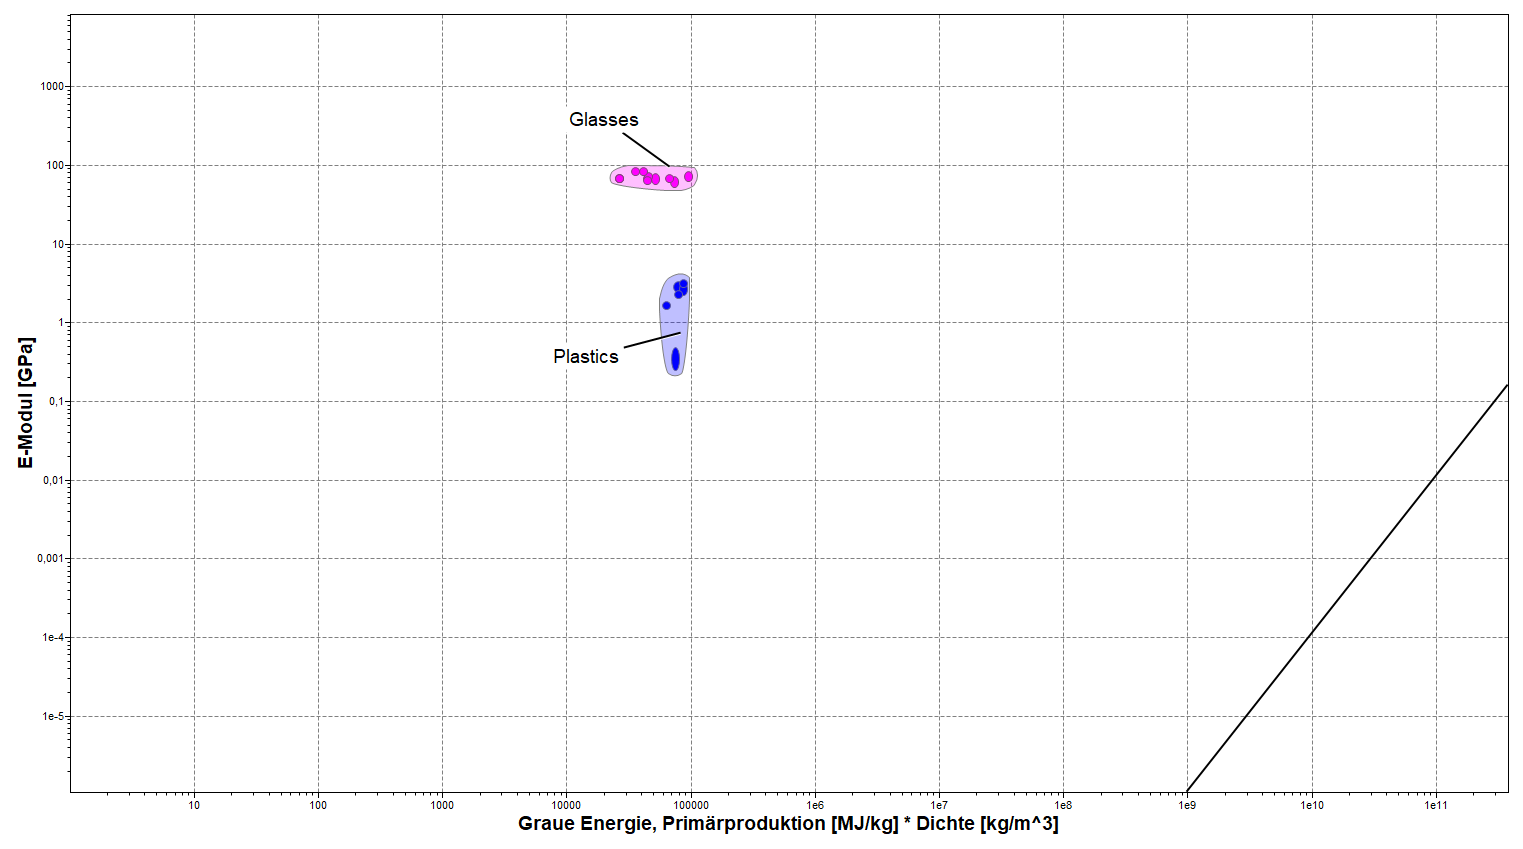
\includegraphics[width=1.0\linewidth]{chapter/Bilder/3_3_2}
	\caption{Caption TODO}
	\label{fig:ces_3_3_2}
\end{figure}
Durch Verschieben der Gerade bleiben die fünf Materialien mit dem höchsten Materialindex übrig (Abb. \ref{fig:ces_3_3_3}).\\
\begin{figure}[H]
	\centering
	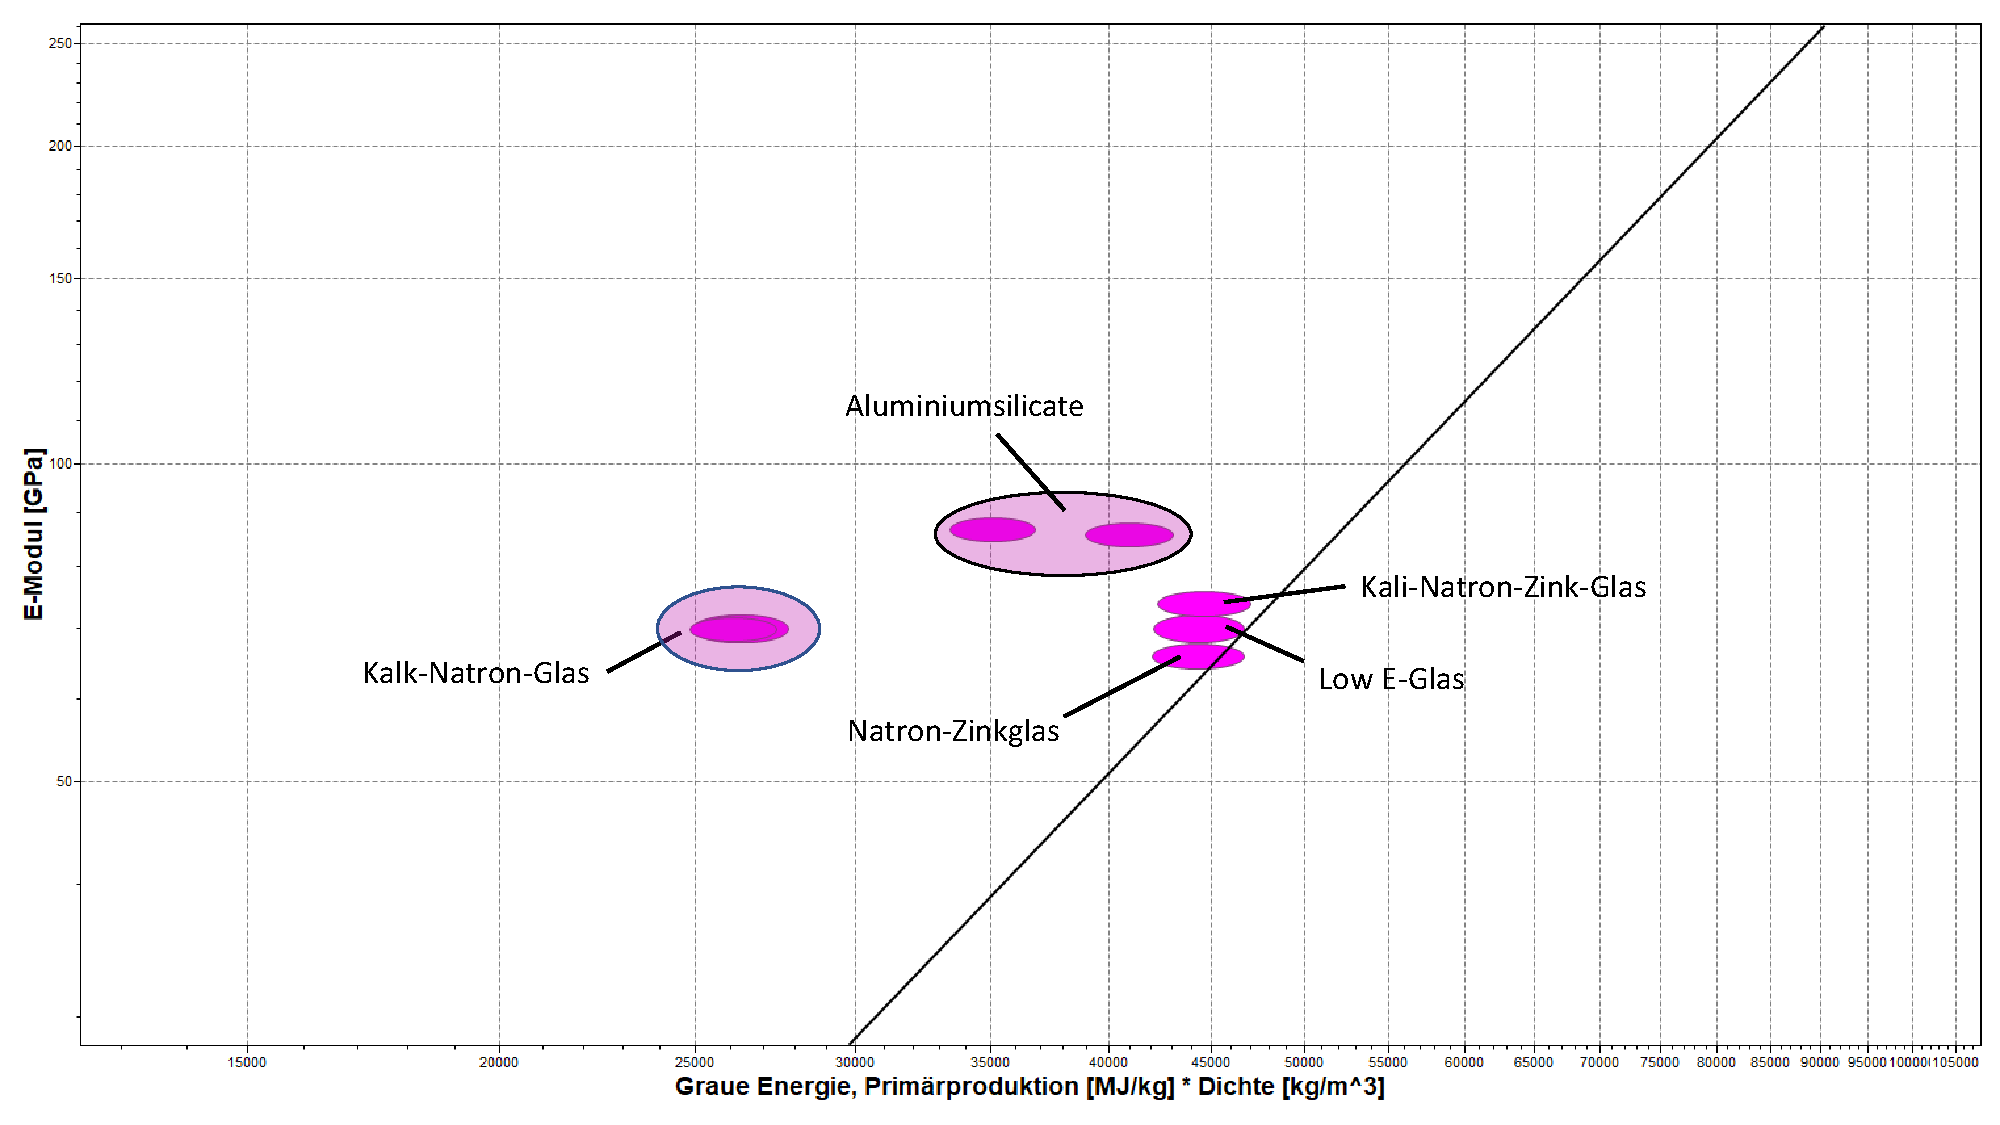
\includegraphics[width=1.0\linewidth]{chapter/Bilder/3_3_3}
	\caption{Caption TODO}
	\label{fig:ces_3_3_3}
\end{figure}
Zu den geeignetsten Materialien gehören:
\begin{itemize}
	\item[1)] Kalk-Natron-Glas (Materialindex: 3,21$\,\times10^{-4}$)
	\item[2)] Aluminiumsilicate (3,2$\,\times10^{-4}$) 
	\item[3)] Kali-Natron-Zink-Glas (1,93$\,\times10^{-4}$)
	\item[4)] Low E-Glas (1,89$\,\times10^{-4}$)
	\item[5)] Natron-Zinkglas (1,84$\,\times10^{-4}$)
\end{itemize}
Kalk-Natron-Glas findet häufig Anwendung zur Fertigung von Behälterglas, wodurch es sich sehr gut als Material für die Lagerungsbehälter eignet.

\section{Aktoren}
Die \textbf{Funktion} der Aktoren ist es die rotatorische Bewegung der Servomotoren in eine translatorische Bewegung umzusetzen und dadurch den Vortrieb eines Schiebers zu erzeugen, wodurch die Tabletten aus der Lagerung geschoben werden. Der prinzipielle Aufbau ist in Abb. ?? gezeigt. Das methodische Selektieren des Werkstoffes für die Baugruppe wird im Folgenden stellvertretend für alle Bauteile am kritischsten Teil, dem Pleuel 2, durchgeführt. Es wirkt auf alle umliegenden Komponenten, die zu dieser Baugruppe gehören, der selbe Belastungszustand, wobei dieser Pleuel im Querschnitt am dünnsten ist, und daher zuerst versagt. Die \textbf{Randbedingungen} hierfür lauten:
\begin{itemize}
	\item Material muss recyclebar sein
	\item Material muss ein guter Isolator sein, bzw. $\rho_e\,>\,10^{19}\,\mu\Omega$cm
	\item Preis $\le\,1,5\,\frac{\text{€}}{\text{kg}}$
\end{itemize}
Das \textbf{Ziel} für die Materialauswahl liegt in der Minimierung der Kosten, um eine hohe Wirtschaftlichkeit des Produktes zu erreichen. Als \textbf{freie Variable} tritt neben der Wahl des Materials die Querschnittfläche des Pleuels auf.\\
Die Gesamtkosten berechnen sich durch:
\begin{equation}
	K\,=\,C_m\,m\,=\,C_m\,\rho\,V\,=\,C_m\,\rho\,A\,l\,.
\end{equation}
Sie können durch Reduzierung der Masse und damit letztendlich durch Reduzierung der Querschnittfläche minimiert werden. Es gilt jedoch, dass mindestens die Zugkraft $F$ ausgehalten werden muss, ohne dass eine plastische Verformung eintritt. Daher folgt
\begin{equation}
	\frac{F}{A}\,\le\,\sigma_y\,,
\end{equation}
wobei $sigma_y$ der Streckgrenze entspricht.
Durch Eliminierung der Querschnittfläche folgt
\begin{equation}
K\,\ge\,C_m\,l\,\,F\,\frac{\rho}{\sigma_y}\,.
\end{equation}
Umstellen liefert die Performance-Gleichung unter Vernachlässigung fester Parameter
\begin{equation}\label{performance34}
P_{CR}^{3.4}\,=\,\frac{1}{K}\,=\,\frac{\sigma_y}{\rho}\,,
\end{equation}
wobei $P_{CR}^{3.4}$ der unter den vorgegebenen Randbedingungen der zu maximierende Materialindex ist. Die graphische Darstellung der Ashby-Methode von Gleichung \ref{performance34} über logarithmierten Achsen sowie der Indexgeraden mit der Steigung 1 ist in Abb. ?? dargestellt.\\
Grafik CES 3-4-1\\
Alle nach Hinzufügen der Randbedingungen übrigen Materialien sind in Abb. ?? dargestellt.\\
Grafik CES 3-4-2\\
Verschieben der Gerade liefert die für den Anwendungsfall am besten geeigneten Materialien (Abb. ??)\\
Grafik CES 3-4-3\\
Die daraus resultierenden Materialien sind:
\begin{itemize}
	\item[1)] Polyesterfasern (Materialindex: 0,364)
	\item[2)] Polyethylenterephtalat (PET, 0,04) 
	\item[3)] Polypropylen (PP, 0,0287)
	\item[4)] Polyethylen (PE - HD, high density, 0,0203)
	\item[5)] Polyethylen (PE - MD, mid density, 0,0157)
\end{itemize}
Dabei haben Polyesterfasern den mit Abstand besten Materialindex. Sie weisen generell sehr gute mechanische Eigenschaften auf, und eignen sich daher am besten für hohe, zyklische Belastung des Bauteils.
%% !TeX encoding = UTF-8
% !TeX root = ../Vitamintablettenspender.tex

\chapter{Ausarbeitung}
%\chapter{Prototypenbau}

%Abbildungsverzeichnis
\listoffigures \thispagestyle{empty} \newpage

%Tabellenverzeichnis
\listoftables \thispagestyle{empty} \newpage

\printbibliography

%Einbinden des Anhangs
\appendix
\chapter{Anhang}
\label{Anhang}
\section{Marktanalyse zu Nahrungsergänzungsmitteln}
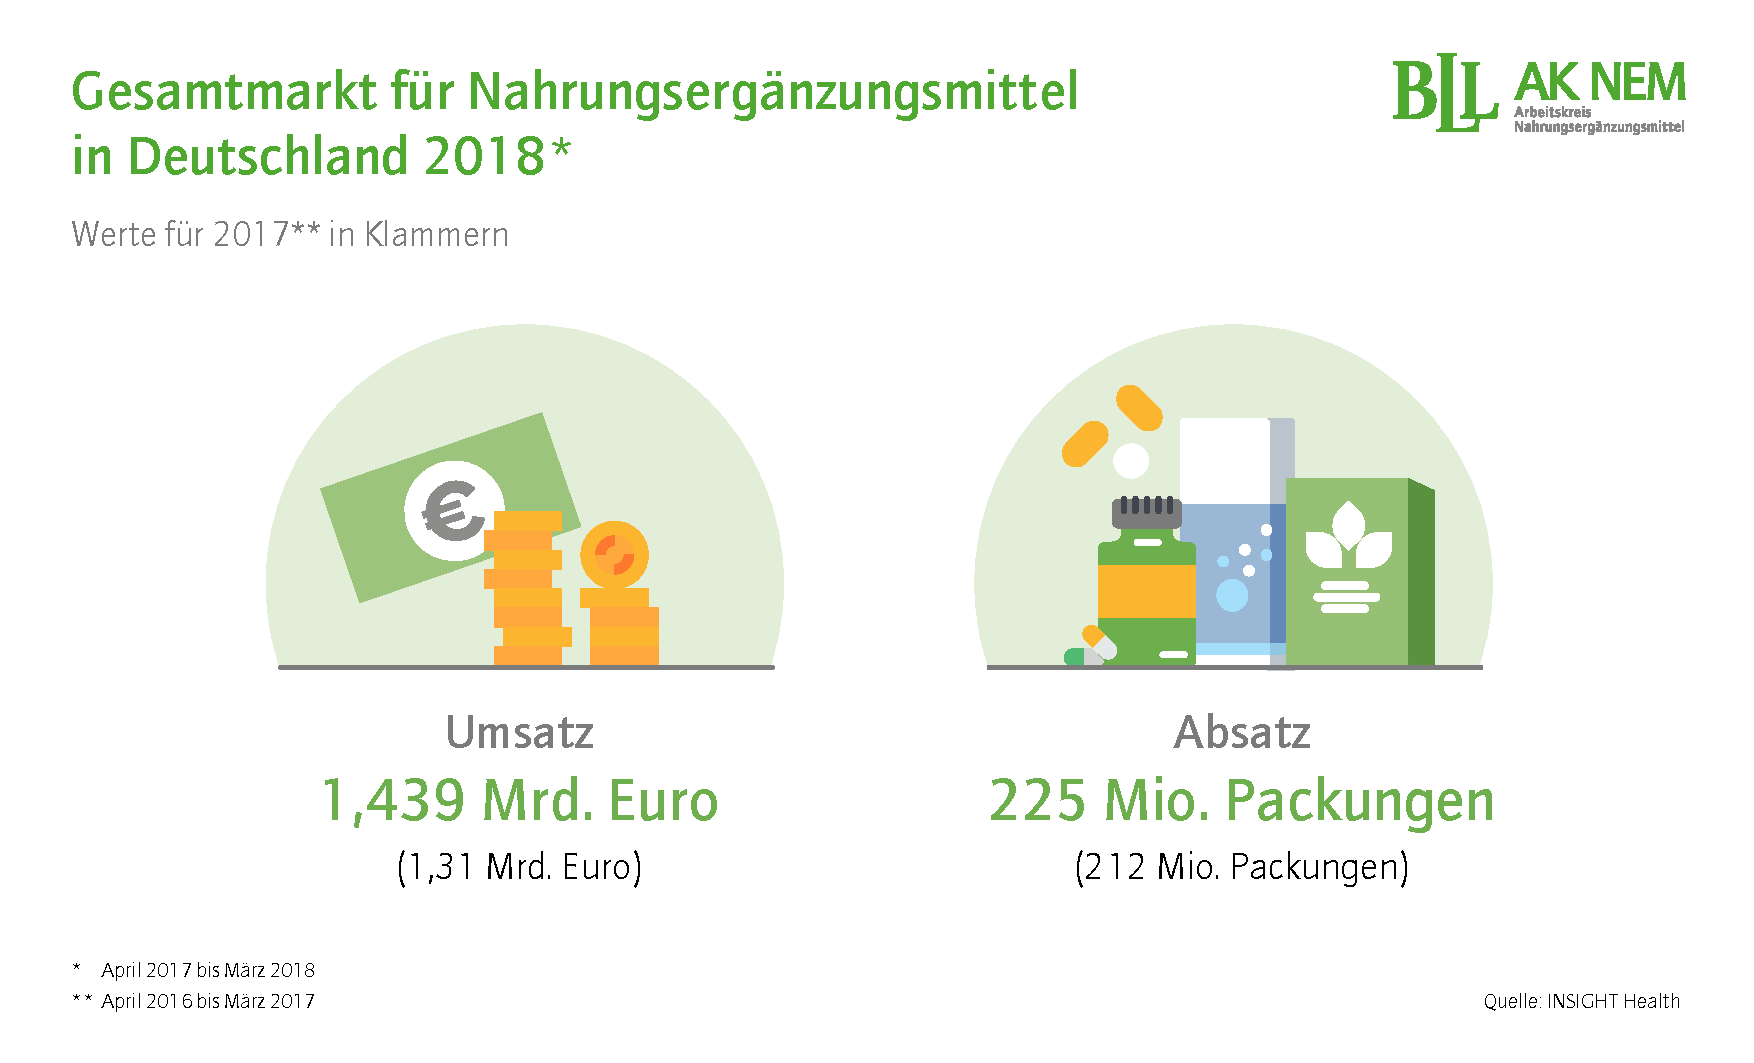
\includepdf[pages={1-3}, nup=1x2]{chapter/Bilder/insighthealth}

\end{document}